%%%%%%%%%%%%%%%%%%%%%%%%%%%%%%%%%%%%%%%%%
% Programming/Coding Assignment
% LaTeX Template
%
% This template has been downloaded from:
% http://www.latextemplates.com
%
% Original author:
% Ted Pavlic (http://www.tedpavlic.com)
%
% Note:
% The \lipsum[#] commands throughout this template generate dummy text
% to fill the template out. These commands should all be removed when 
% writing assignment content.
%
% This template uses a Perl script as an example snippet of code, most other
% languages are also usable. Configure them in the "CODE INCLUSION 
% CONFIGURATION" section.
%
%%%%%%%%%%%%%%%%%%%%%%%%%%%%%%%%%%%%%%%%%

%----------------------------------------------------------------------------------------
%	PACKAGES AND OTHER DOCUMENT CONFIGURATIONS
%----------------------------------------------------------------------------------------

\documentclass{article}

\usepackage{fancyhdr} % Required for custom headers
\usepackage{lastpage} % Required to determine the last page for the footer
\usepackage{extramarks} % Required for headers and footers
\usepackage[usenames,dvipsnames]{color} % Required for custom colors
\usepackage{graphicx} % Required to insert images
\usepackage{listings} % Required for insertion of code
\usepackage{courier} % Required for the courier font
\usepackage{pgfgantt}

% Margins
\topmargin=-0.45in
\evensidemargin=0in
\oddsidemargin=0in
\textwidth=6.5in
\textheight=9.0in
\headsep=0.3in

\linespread{1.1} % Line spacing

% Set up the header and footer
\pagestyle{fancy}
\lhead{\homeworkProblemName} % Top left header
\chead{\hmwkTitle} % Top center head
\rhead{\hmwkClass } % Top right header
\lfoot{} % Bottom left footer
\cfoot{} % Bottom center footer
\rfoot{Page\ \thepage\ of\ \protect\pageref{LastPage}} % Bottom right footer
\renewcommand\headrulewidth{0.4pt} % Size of the header rule
\renewcommand\footrulewidth{0.4pt} % Size of the footer rule

\setlength\parindent{0pt} % Removes all indentation from paragraphs

%----------------------------------------------------------------------------------------
%	CODE INCLUSION CONFIGURATION
%----------------------------------------------------------------------------------------

\definecolor{MyDarkGreen}{rgb}{0.0,0.4,0.0} % This is the color used for comments
\lstloadlanguages{Java} % Load Java syntax for listings, for a list of other languages supported see: ftp://ftp.tex.ac.uk/tex-archive/macros/latex/contrib/listings/listings.pdf
\lstset{language=Java, % Use Java in this example
        frame=none, % Single frame around code
        basicstyle=\small\ttfamily, % Use small true type font
        keywordstyle=[1]\color{Blue}\bf, % Perl functions bold and blue
        keywordstyle=[2]\color{Purple}, % Perl function arguments purple
        keywordstyle=[3]\color{Blue}\underbar, % Custom functions underlined and blue
        identifierstyle=, % Nothing special about identifiers                                         
        commentstyle=\usefont{T1}{pcr}{m}{sl}\color{MyDarkGreen}\small, % Comments small dark green courier font
        stringstyle=\color{Purple}, % Strings are purple
        showstringspaces=false, % Don't put marks in string spaces
        tabsize=8, % 5 spaces per tab
        %
        % Put standard Perl functions not included in the default language here
        morekeywords={rand},
        %
        % Put Perl function parameters here
        morekeywords=[2]{on, off, interp},
        %
        % Put user defined functions here
        morekeywords=[3]{test},
       	%
        morecomment=[l][\color{Blue}]{...}, % Line continuation (...) like blue comment
        numbers=left, % Line numbers on left
        firstnumber=1, % Line numbers start with line 1
        numberstyle=\tiny\color{Blue}, % Line numbers are blue and small
        stepnumber=100 % Line numbers go in steps of 5
}


%----------------------------------------------------------------------------------------
%	DOCUMENT STRUCTURE COMMANDS
%	Skip this unless you know what you're doing
%----------------------------------------------------------------------------------------

% Header and footer for when a page split occurs within a problem environment
\newcommand{\enterProblemHeader}[1]{
\nobreak\extramarks{#1}{#1}\nobreak
\nobreak\extramarks{#1}{#1}\nobreak
}

% Header and footer for when a page split occurs between problem environments
\newcommand{\exitProblemHeader}[1]{
\nobreak\extramarks{#1}{#1 continued on next page\ldots}\nobreak
\nobreak\extramarks{#1}{}\nobreak
}

\setcounter{secnumdepth}{0} % Removes default section numbers
\newcounter{homeworkProblemCounter} % Creates a counter to keep track of the number of problems

\newcommand{\homeworkProblemName}{}
\newenvironment{homeworkProblem}[1][
 \arabic{homeworkProblemCounter}]{ % Makes a new environment called homeworkProblem which takes 1 argument (custom name) but the default is "Problem #"
\stepcounter{homeworkProblemCounter} % Increase counter for number of problems
\renewcommand{\homeworkProblemName}{#1} % Assign \homeworkProblemName the name of the problem
\section{\homeworkProblemName} % Make a section in the document with the custom problem count
\enterProblemHeader{} % Header and footer within the environment
}{
\exitProblemHeader{} % Header and footer after the environment
}

\newcommand{\problemAnswer}[1]{ % Defines the problem answer command with the content as the only argument
\noindent\framebox[\columnwidth][c]{\begin{minipage}{0.98\columnwidth}#1\end{minipage}} % Makes the box around the problem answer and puts the content inside
}

\newcommand{\homeworkSectionName}{}
\newenvironment{homeworkSection}[1]{ % New environment for sections within homework problems, takes 1 argument - the name of the section
\renewcommand{\homeworkSectionName}{#1} % Assign \homeworkSectionName to the name of the section from the environment argument
\subsection{\homeworkSectionName} % Make a subsection with the custom name of the subsection
\enterProblemHeader{\homeworkProblemName\ [\homeworkSectionName]} % Header and footer within the environment
}{
\enterProblemHeader{\homeworkProblemName} % Header and footer after the environment
}


%----------------------------------------------------------------------------------------
%	NAME AND CLASS SECTION
%----------------------------------------------------------------------------------------

\newcommand{\hmwkTitle}{Group Project: A Fault Tolerant Voting Service} % Assignment title
\newcommand{\hmwkDueDate}{We're not even sure} % Due date
\newcommand{\hmwkClass}{COMP30220} % Course/class
\newcommand{\hmwkClassTime}{Distributed Systems} % Class/lecture time
\newcommand{\hmwkClassInstructor}{Dr. Rem Collier} % Teacher/lecturer
\newcommand{\hmwkAuthorName}{Group Name: Lamp + Gary} % Your name

%----------------------------------------------------------------------------------------
%	TITLE PAGE
%----------------------------------------------------------------------------------------

\title{
\vspace{2in}
\textmd{\textbf{\hmwkClass:\ \hmwkClassTime}}\\
\normalsize\
\vspace{0.1in}\large{\textit{\hmwkClassInstructor}}\\
\vspace{0.2in}
\textmd{\textbf{\hmwkTitle}}\\
\small{Due\ on\ \hmwkDueDate}\\
\vspace{.5in}
}

\author{\textbf{\hmwkAuthorName}\\
Joe Duffin - 13738019
\\Niamh Kavanagh - 12495522
\\Edwin Keville - 13718661
\\Gary Mac Elhinney - XXXXXXXX
}

\date{} % Insert date here if you want it to appear below your name

%----------------------------------------------------------------------------------------

\begin{document}
%\begin{titlepage}
%\maketitle
%\thispagestyle{empty}
%\end{titlepage}

%\newpage
%----------------------------------------------------------------------------------------
%	TABLE OF CONTENTS
%----------------------------------------------------------------------------------------

%\setcounter{tocdepth}{1} % Uncomment this line if you don't want subsections listed in the ToC

%\newpage
%\tableofcontents
%\newpage

%----------------------------------------------------------------------------------------

\begin{homeworkProblem}[Use Cases]
Here we present 5 different sets of screen shots demonstrating different stages of a use of the distributed voting service. The client can choose to repeatedly vote for one of four people or request a printout of the current standings. These use cases demonstrate the high availablity of our service, and how the client is for all intent and purpose unaware of what it going on server side.

\begin{homeworkSection}{Leader Election}

In the below set of terminals 3 servers were started almost instantaniously. It is evident how Server5316 can't find an instance of the jgUDDI service registry is not present so it starts it. It publishes its self and then before its election timer runs out it has identified that two other servers have been started. Its election timer then runs out and it becomes a candidate, requests votes, recieves votes and then becomes the new leader. "Badump" indicates that it is sending heart beat messages.
\begin{center}
Server5316\\
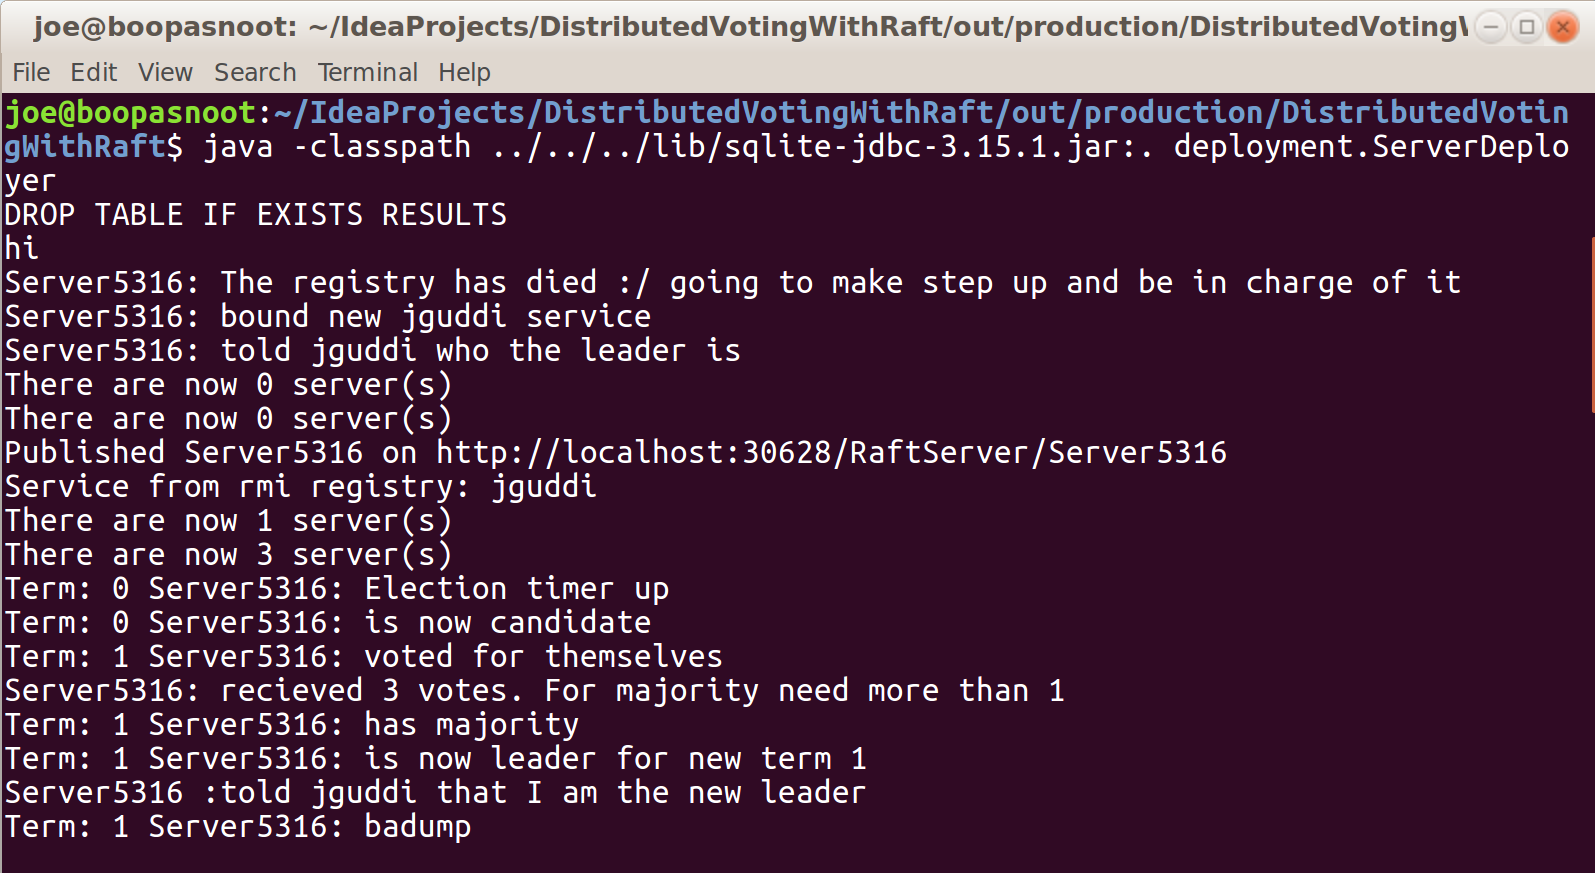
\includegraphics[width=0.95\columnwidth]{election1}
\end{center}
\newpage
It is evident in the other two terminals (Server9547 and Server5810) that they find the jgUDDI service hosted by Server5316, vote for Server5316 and then start to recieve heart beat messages from Server5316. If a client was to vote, the transaction log would be embedded in the heart beat message.
\begin{center}
Server9547\\
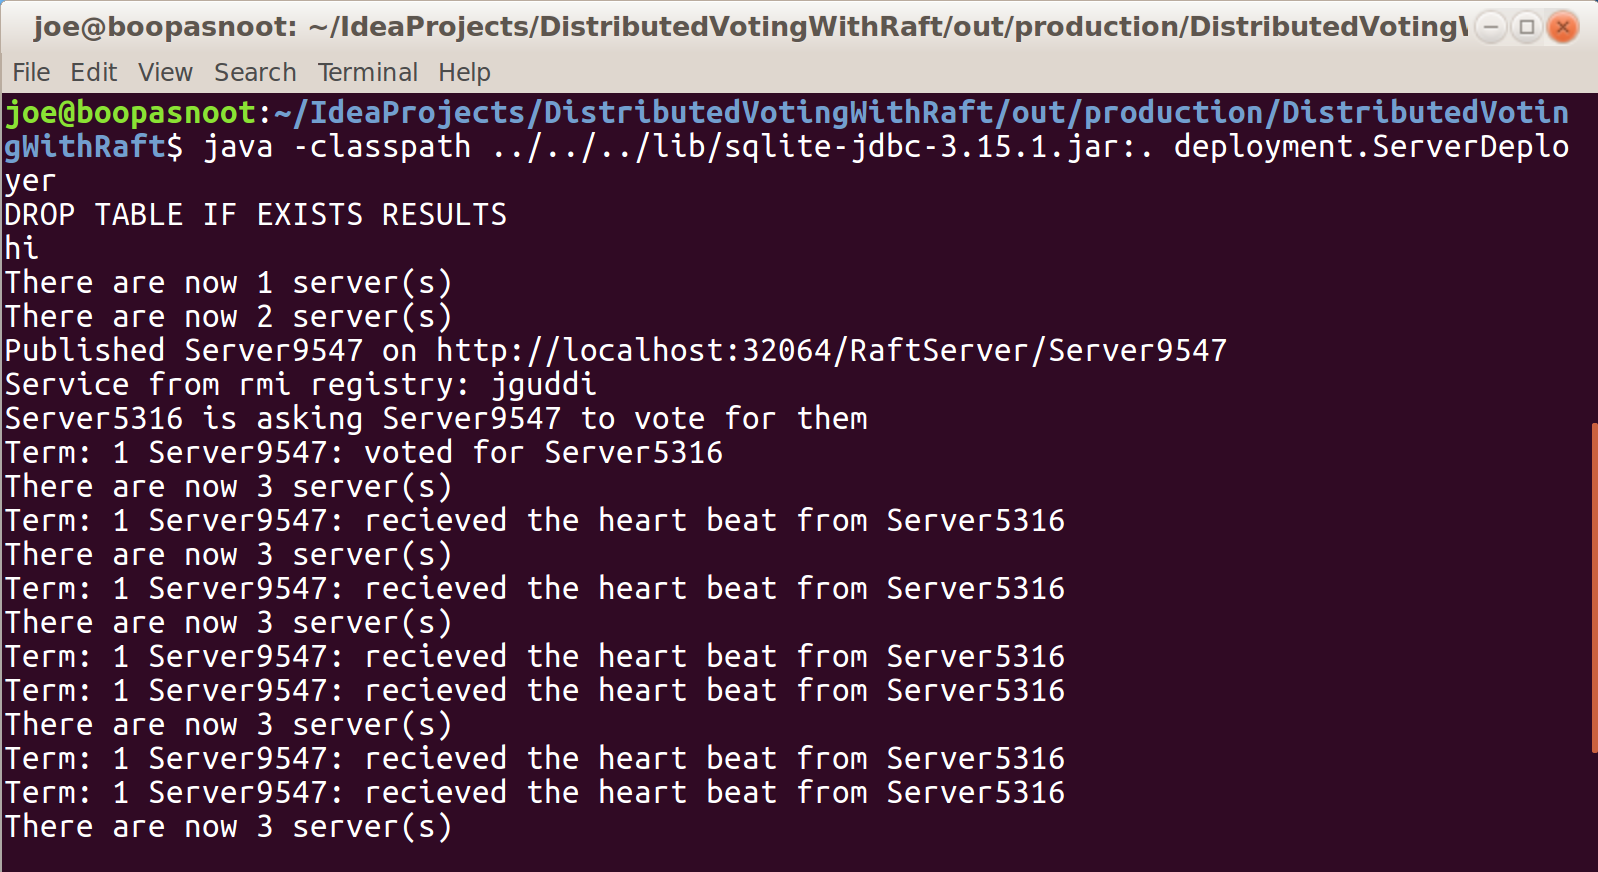
\includegraphics[width=0.95\columnwidth]{election2}
\end{center}
\begin{center}
Server5810\\
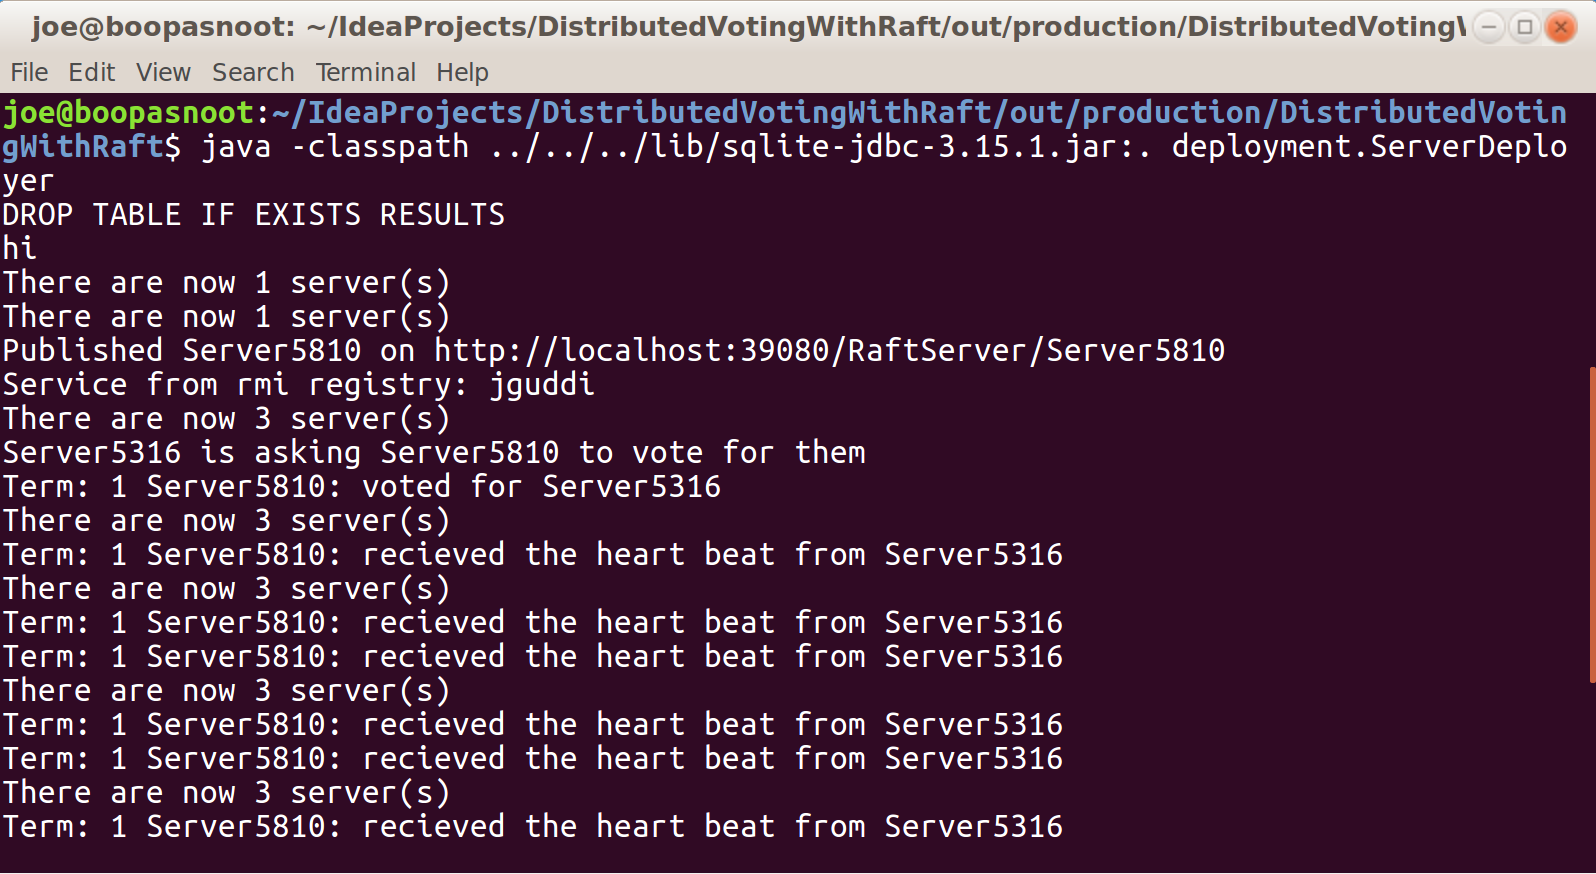
\includegraphics[width=0.95\columnwidth]{election3}
\end{center}

\end{homeworkSection}
\newpage
\begin{homeworkSection}{Client Interaction}
Here we present two terminals, a follower and the client. The client has made three votes and then requested the current standings. The client always votes to the current leader which is Server2538.
\begin{center}
Client\\
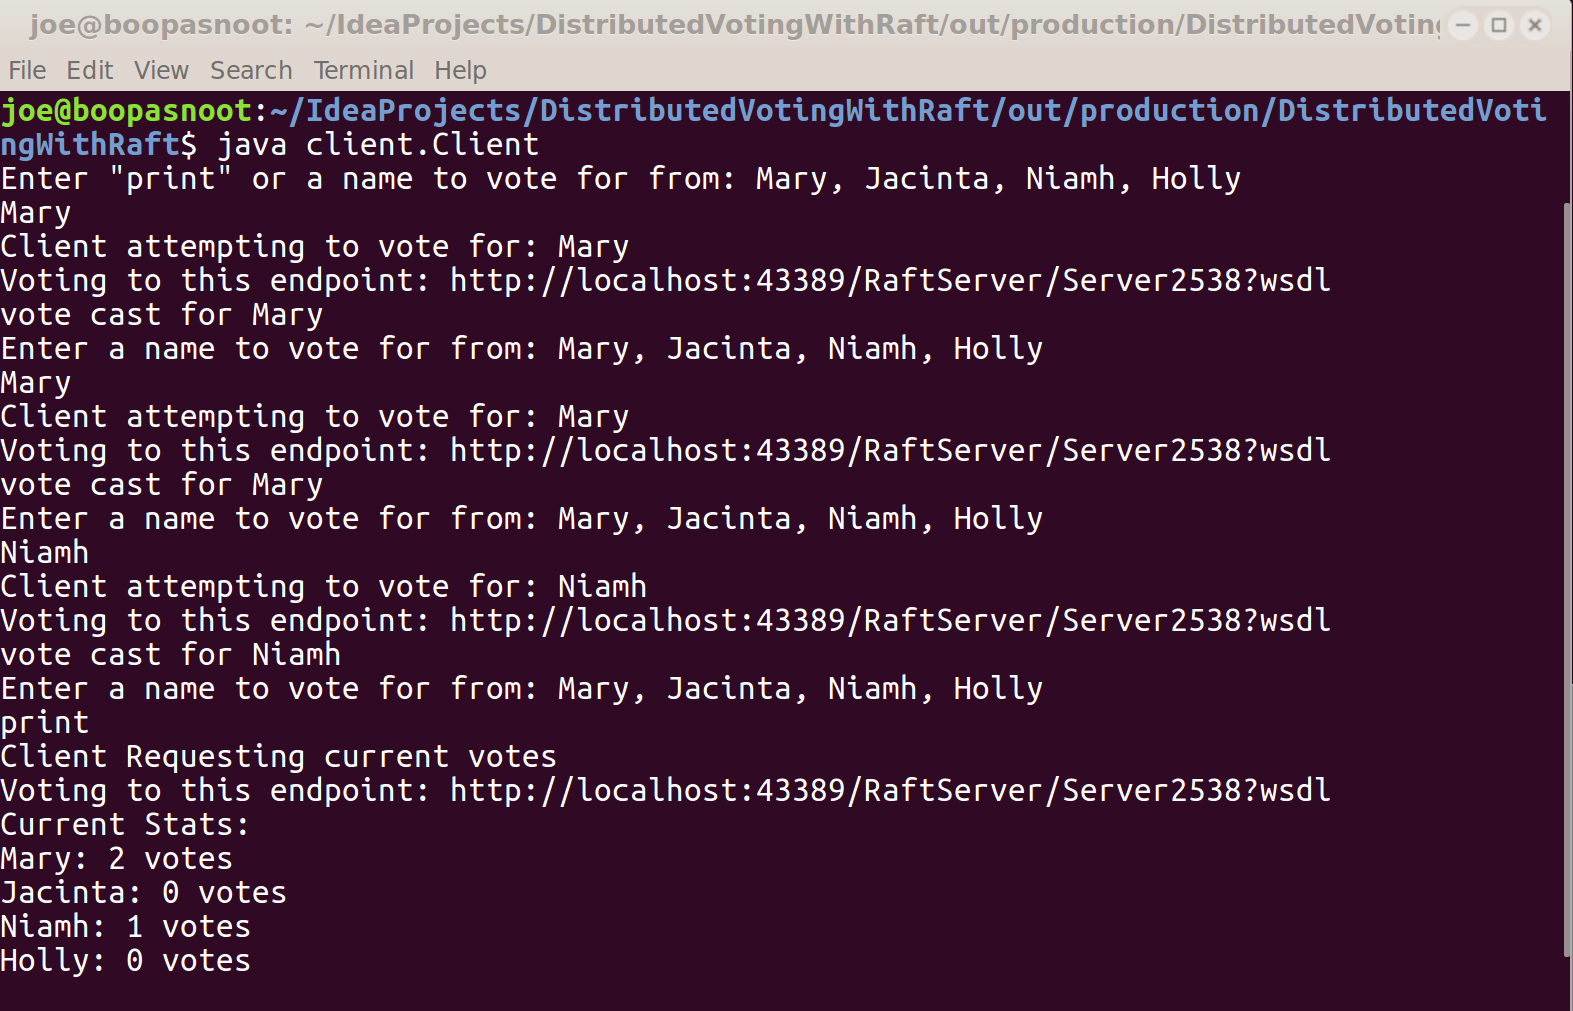
\includegraphics[width=0.95\columnwidth]{clientVote1}
\end{center}
The servers terminal shows the recieved heart beats, the continued checks for other servers from the jgUDDI service and the vote data which gets passed to the coordinator.
\begin{center}
Server8036\\
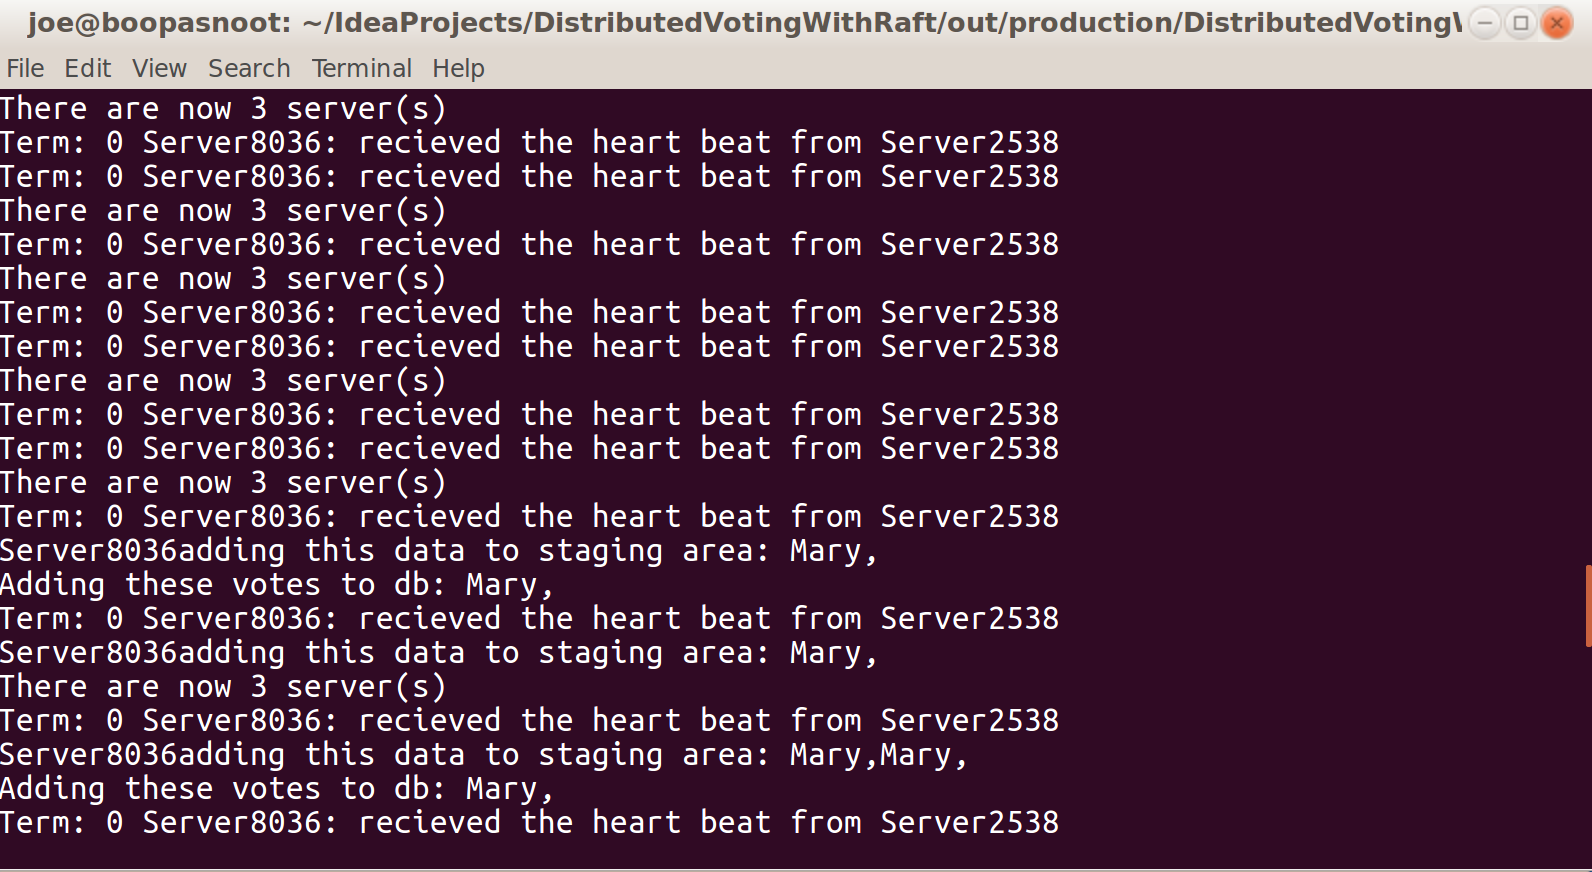
\includegraphics[width=0.95\columnwidth]{clientVote2}
\end{center}
\end{homeworkSection}
\newpage
\begin{homeworkSection}{Leader Crash}
The following terminal shows that Server234s reaction to a leader crash. Server234 restarted jgUDDI and repopulated its with current information and removed the dead enpoint (that belonged to the old leader that crashed). It then requests votes and although there is an initial "blip" in service it eventually gets the needed votes to become the new leader and starts sending out heart beat messages. The downtime of the service was minimal.
\begin{center}
Server234\\
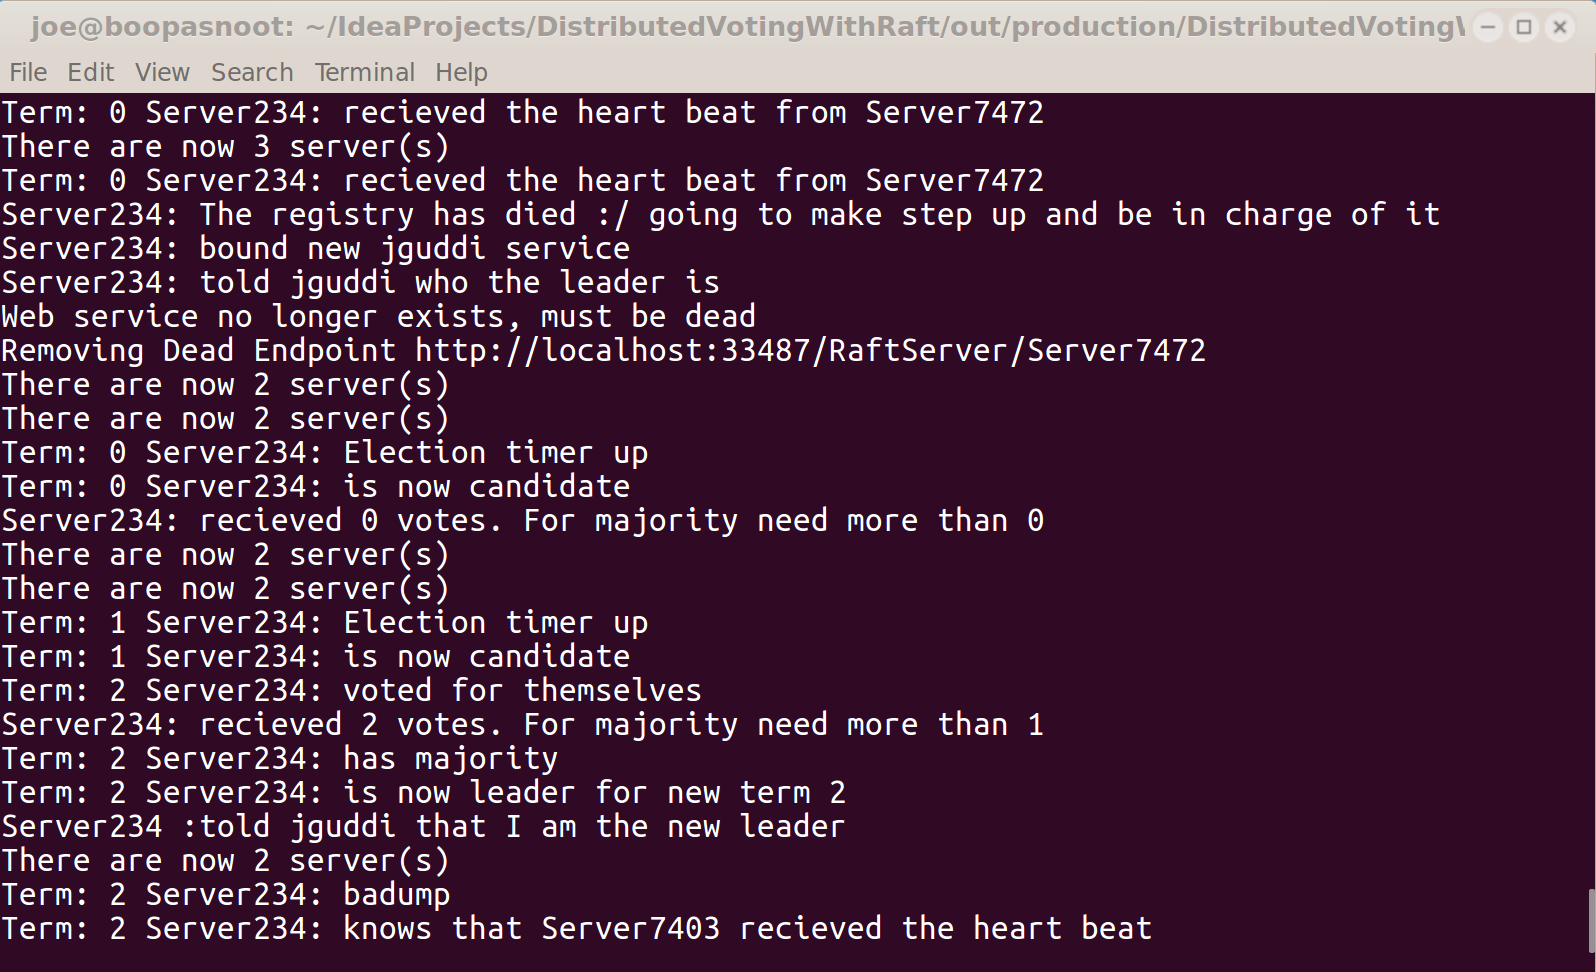
\includegraphics[width=0.9\columnwidth]{crash1}
\end{center}

During the switchover Server7403 attempts to become the new leader but failed. It ultimately votes for Server234 and becomes its follower.
\begin{center}
Server7403\\
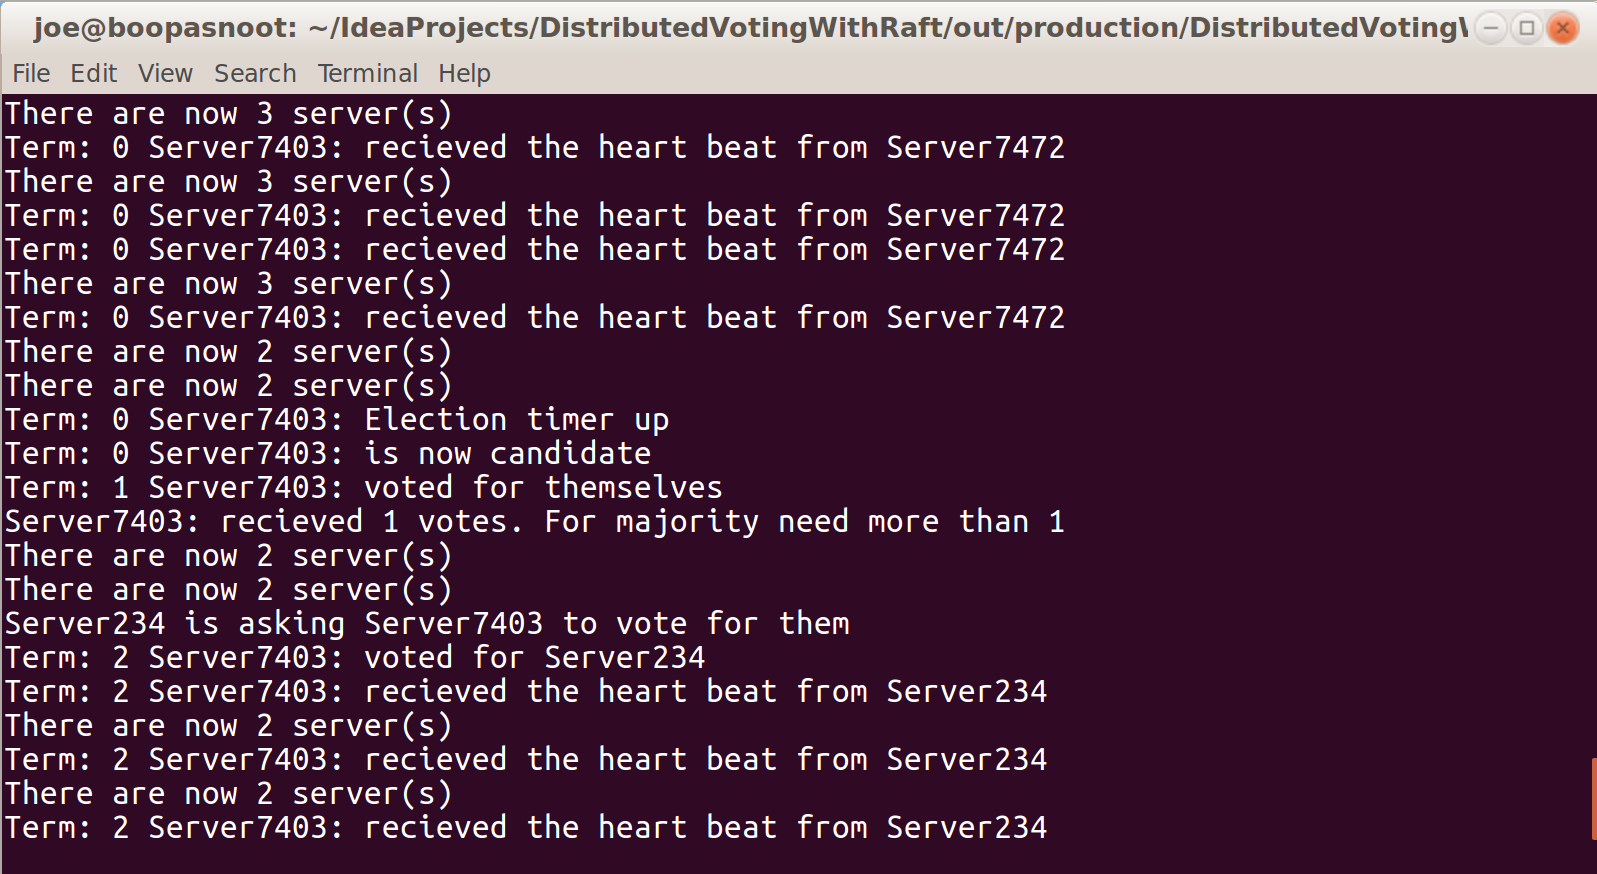
\includegraphics[width=0.9\columnwidth]{crash2}
\end{center}
\newpage
\end{homeworkSection}

\begin{homeworkSection}{New Server Coming Online}
Here we present the output of a server that was brought online at a later time to the service start time. Many votes have been cast at this point. The new server is instantly updated with the latest transaction log from the current leader (Server1041) and it updates its database accordingly.

\begin{center}
Server1117\\
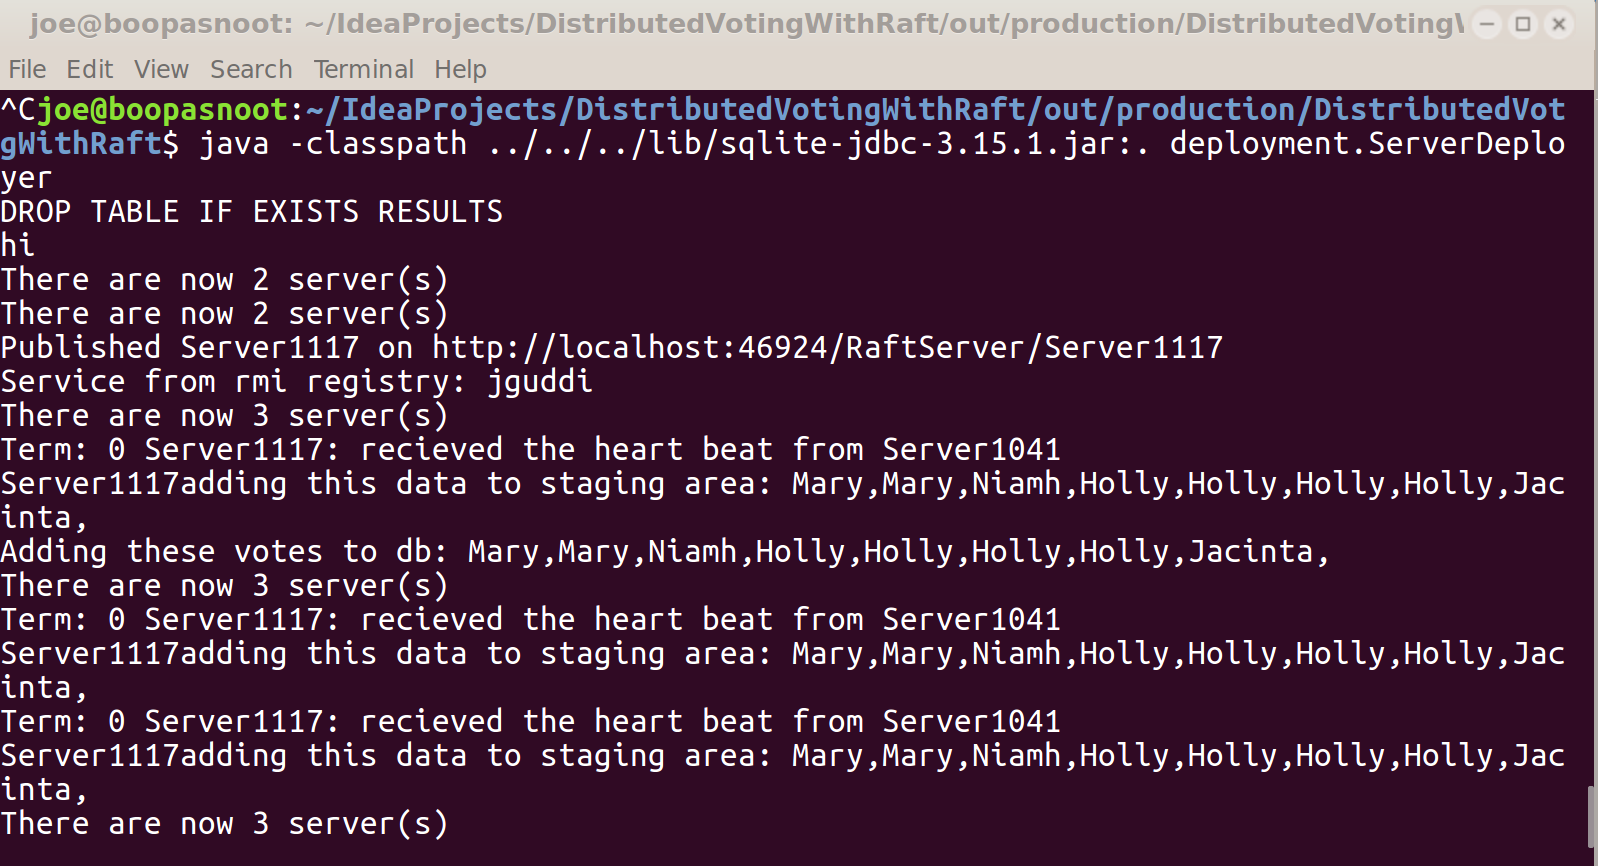
\includegraphics[width=0.9\columnwidth]{new1}
\end{center}


\end{homeworkSection}
\newpage
\begin{homeworkSection}{The Worst Case Scenario}
Here we present the robustness of our distributed voting service. The situation presented is as follows.
\begin{enumerate}
\item Many votes have been cast.
\item The leader has crashed.
\item Another server has been brought online.
\item All servers bar the most recently started server have crashed.
\end{enumerate}

It is evident in the client output that everything is fine from it's point of view. The only difference is that it is now requesting standings from a different server endpoint. This printout is only for the point of demonstration and a user of the client service would be ignorant to the change in leader endpoint.

\begin{center}
Client\\
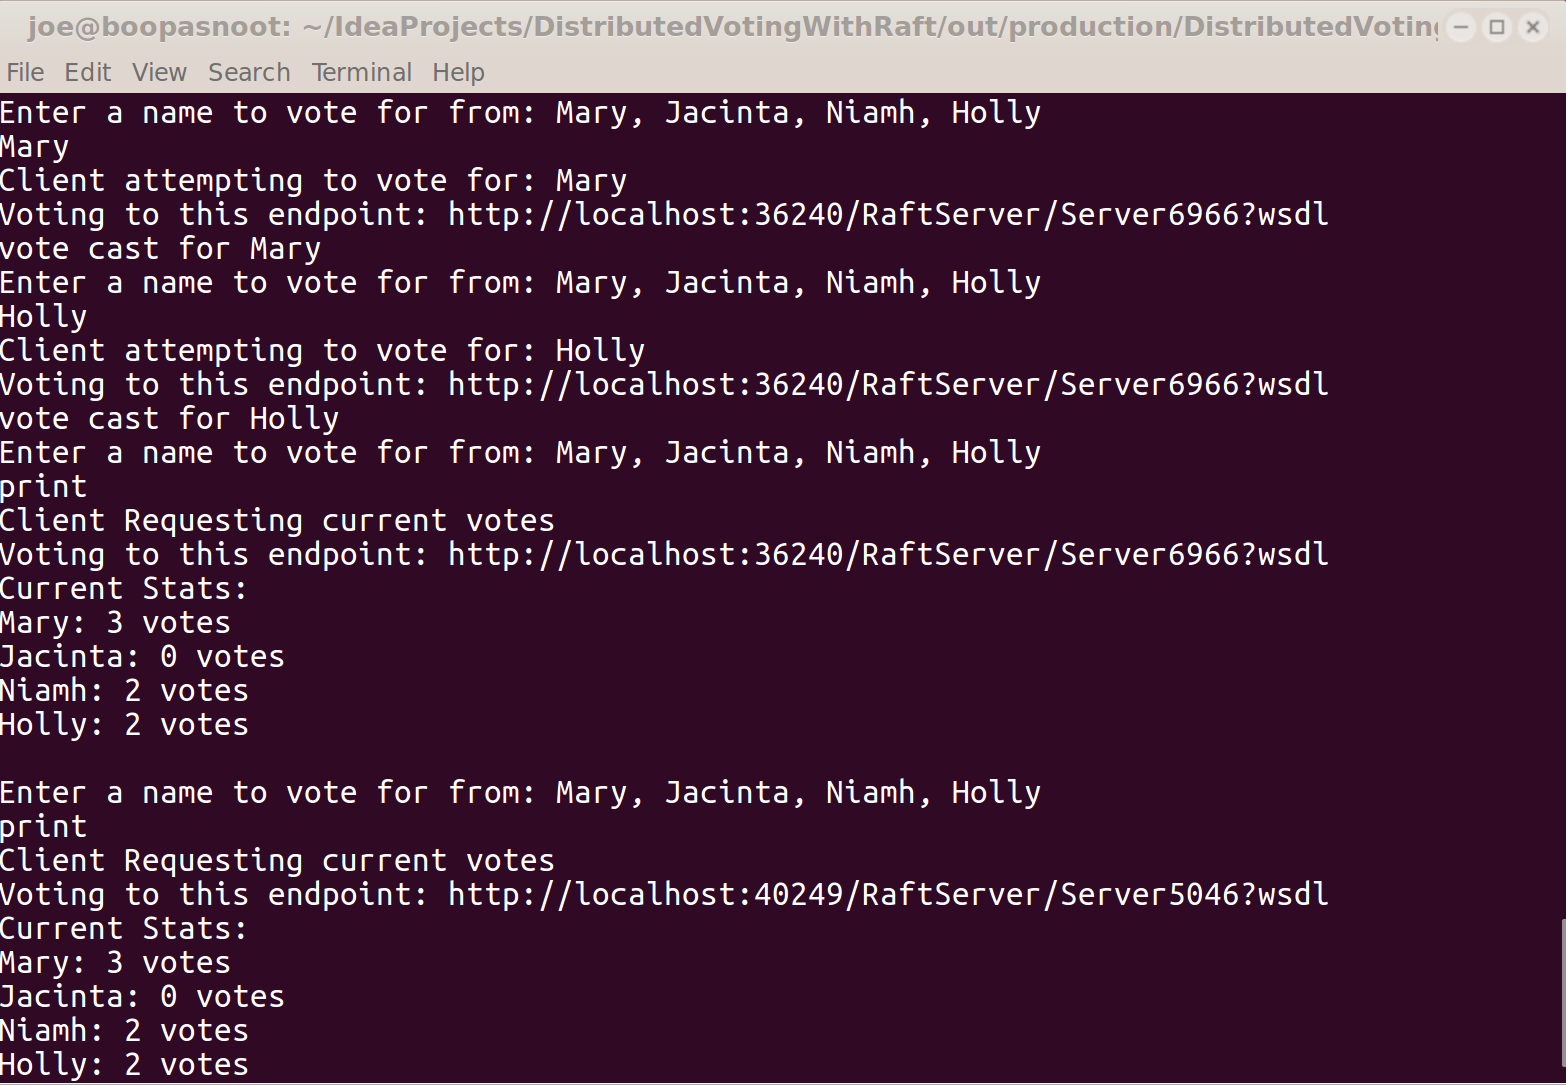
\includegraphics[width=0.95\columnwidth]{worst1}
\end{center}

\end{homeworkSection}

\newpage
\end{homeworkProblem}
%----------------------------------------------------------------------------------------




\end{document}